

\paragraph{} In this chapter we shall introduce and detail a prototype implementation of a modular, SGX-protected \textit{reference monitor} --- \textsc{Citadel}. First, its necessity will be motivated, and the challenges faced discussed. Then, the three-part architecture will be explained, relating various design decisions to the DIFC model it provides. A discussion about the architecture's performance and effectiveness is provided in §~\ref{sec:eval}.

\section{Motivation}
\paragraph{} Since its introduction in a 1972 report from Anderson~\cite{reference-monitor}, the reference monitor concept has time and again proved to be a reliable workhorse for a plethora of security models. It does not refer to any exact policy, nor limit itself to any particular implementation --- it's abstractness is one of its greatest strengths, reserving any judgement about what policy is \textit{appropriate} in a particular setting.~\cite{irvine-rm}

\paragraph{Fundamental Properties of a Reference Monitor}

\begin{itemize}
    \item \textit{Always invoked.} Every access to the system must be mediated to guarantee that adversaries are unable to bypass the system's security policies.
    \item \textit{Evaluable.} It ``must be small enough to be subject to analysis and tests, the completeness of which can be assured'';~\cite{reference-monitor} to be trustworthy, it must be \textit{auditable}, with, ideally, a restricted TCB.
    \item \textit{Tamper proof.} To ensure that an attacker cannot disable the access control and authorisation steps mandated by the security policy, the integrity of a reference monitor cannot be in question.
\end{itemize}

\paragraph{} No computer system is every completely secure, and Linux is no exception. Having grown by a 1.7 million lines of code (LoC) in the past year alone, to stand at 27.8 million LoC in total,\footnote{\url{https://www.theregister.com/2020/01/06/linux\_2020\_kernel\_systemd\_code/}} bugs are inevitable --- almost 2000 have been reported in the past year,\footnote{\url{https://bugzilla.kernel.org/}} and 662 \textit{severe} bugs are still outstanding.\footnote{\url{https://www.cvedetails.com/product/47/Linux-Linux-Kernel.html}} In this context we must question whether Linux alone can provide a reference monitor implementation the guarantees it requires,~\cite{Lipp2018MeltdownRK, 10.5555/2831143.2831164} thus motivating the use of SGX.

\paragraph{} Applying SGX to this problem brings two attractive benefits;
\begin{itemize}
    \item The system's IFC policy can be evaluable both during offline analysis and online using \textit{attestation}, helping other enclaves' confidence in the underlying system.
    \item SGX's hardware protections are very capable at defending a reference monitor's state, even if adversaries have ring-0 privilege or in the presence of a kernel bug.
\end{itemize}

\section{Challenges}

\begin{figure}[]
    \centering
    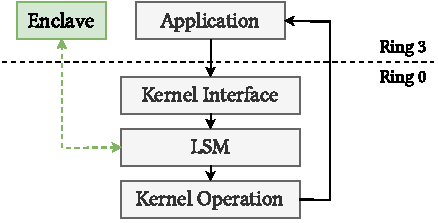
\includegraphics[width=0.48\linewidth]{figures/SGX-EnclaveIntegration.pdf}
    \caption{Abstract \textit{syscall} control flow route. Grey components show the natural Linux design. Green additions highlight the externalised enclave LSM component.}
    \vspace{5mm}
    \label{fig:sgx-abstract-integration}
\end{figure}

\paragraph{} The natural location for a reference monitor is embedded directly in the kernel, in the path of \textit{syscalls'} control flows --- this is provided by the LSM framework. \textit{CamFlow} does exactly this, silently tagging processes and other entities as they are encountered by the kernel, additionally providing an external LSM-interface for any active changes. An SGX enclave is incompatible with this workflow however (§~\ref{sec:sgx-no-kernel-mode}), as it cannot execute alongside kernel code. Thus a major, unavoidable design decision is that the reference monitor must be distributed across rings 0 and 3 --- an enclave \textit{policy} component, and an LSM for \textit{enforcement}.

\paragraph{} The disruption this change causes could have the potential to severely impact performance; Figure~\ref{fig:sgx-abstract-integration} highlights the significant change to overall control flow. Most notably, externalising part of the LSM to an enclave forces, in the worst case, an additional pair of context switches for each \textit{syscall}.

\paragraph{} Given a ring-3 component is unavoidable, the question becomes how to minimise the overhead caused by its integration, all while maintaining \textit{safety} (every operation must be mediated). This problem is reminiscent of the ones that inspired the development of \textit{exokernels}~\cite{10.1145/224056.224076} --- both the drawbacks and opportunities of those approaches apply here.~\cite{10.1145/269005.266644} \textcolor{red}{More detail about why.}

\paragraph{} Two architectures, as illustrated in Figure~\ref{fig:sgx-integration}, were initially considered. 

\begin{enumerate}
    \item An \textit{isolated} extension of the LSM. Only the security implementation communicates with the \textit{policy} enclave, acting as a na\"{i}ve reimplementation of a fully self-contained LSM using an additional kernel module as an I/O relay.
    \item An \textit{integrated} userspace service, through which permission is \textit{requested} ahead of time and decisions stored in the LSM before being needed. Back flow of information is facilitated asynchronously, but an additional kernel relay is not required.
\end{enumerate}



\begin{figure}[]
    \centering
    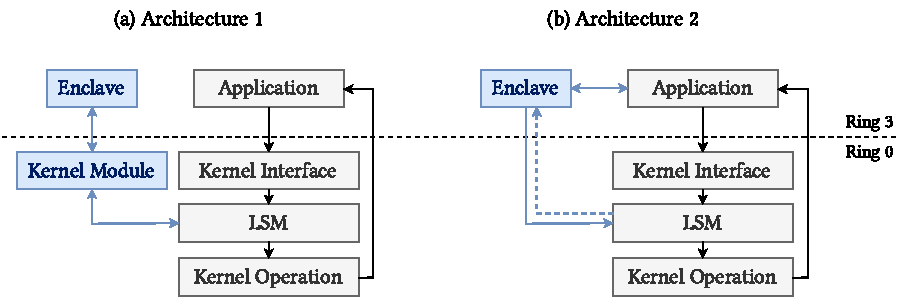
\includegraphics[width=0.98\linewidth]{figures/SGX-EnclaveIntegration-Design}
    \caption{}
    \vspace{2mm}
    \label{fig:sgx-integration}
    \vspace{5mm}
\end{figure}

\paragraph{}\textit{Architecture 1} can be implemented without changing the base IFC model presented in §~\ref{sec:ifc-modelling}, easing potential concerns regarding correctness and safety. However it adds significant overhead to the critical sections~\cite{Dubois1988SynchronizationCA} of core LSM functions, in most cases while the kernel holds locks for various objects being accessed.

\paragraph{} \textit{Architecture 2} is more flexible, requiring all negotiation be conducted ahead of time, and importantly, without leaving userspace: any overhead only impacts the application, leaving the kernel's critical sections to execute with minimal interference. A notable downside, however, is that the system's security model will need to be extended to accommodate the fact that \textit{policy decisions and enforcement are no longer one and the same}.

\paragraph{} Preliminary experiments showed that the performance of the two architectures were similar in light workloads, but \textit{Architecture 1} degrades significantly in the presence of any resource contention. Additionally, as will be explained in §~0.0, the dependence on a kernel module conflicts with the desired constrained TCB of the system. For these reasons \textit{Architecture 2} was chosen for the remainder of development.

\paragraph{} An additional challenge is one of incomplete information --- the enclave will not be privy to internal kernel datastructures such as \texttt{task\_struct}, which will store the taint and capabilities of processes. A potential solution would be to implement a request---response model via a custom kernel interface for any queries, though the performance impact would be severe, requiring additional context switches. The approach adopted instead (§~0.0) uses inference based on partial information an enclave has. Any solution must be trustworthy and safe, and malicious entities must not be able to exploit any \textit{eventually consistent} components.~\cite{10.1145/1435417.1435432}

\paragraph{} As a final comment, it must be noted that SGX is not without its flaws; §~5.X discusses this and its impact on the project.


% ---------------

\section{The \textsc{Citadel} IFC Model}

\paragraph{} Before work on the final \textsc{Citadel} implementation began, we constructed a formalisation describing the distributed nature of its design. A model helps reason about the safety and correctness of the final system, and provides the notation to properly discuss its features. Our model, which will now be presented, directly extends the one presented in §~\ref{sec:ifc-modelling}.

\subsection{Reservations}

\paragraph{} Previously we had defined the concept of a \textit{safe flow}, $A \rightarrow B$, which underpins the heart of our IFC restrictions. In previous works permission to perform an operation is granted while \textit{implicitly} considering \textit{how} the flow is to take place (\ref{eqn:res-1}). An isolated \textit{enforcement} component does not understand the concept of \textit{flows}, forcing policy decisions to be defined \textit{explicitly}; \textsc{Citadel} uses \textit{reservations} for this purpose (\ref{eqn:res-2}). This distinction is simple but very important when introducing \textit{laziness} and other optimisations between the two halves of the reference monitor.

\begin{equation}\label{eqn:res-1}
    \textit{operation} \rightarrow \boxed{\textit{reference monitor}} \xrightarrow{\;\;\textit{decision}\;\;} \{0,1\}
\end{equation}
\vspace{-3mm}
\begin{equation}\label{eqn:res-2}
    \textit{operation} \rightarrow \boxed{\textit{policy}\; \xrightarrow{\;\;\textit{reservation}\;\;} \;\textit{enforcement}} \xrightarrow{\;\;\textit{decision}\;\;} \{0,1\}
    \vspace{3mm}
\end{equation}


\paragraph{} Let $\Omega$ be the set of all operations mediated by the reference monitor, for example \texttt{file\_read} or \texttt{socket\_open}. Also, let us define $\mathcal{R}$, the set of all \textit{reservations}, as follows.\footnote{Recalling that $\mathcal{T}$ is the set of all tags.}

\newcommand{\powerset}{\raisebox{.15\baselineskip}{\Large\ensuremath{\wp}}}
\vspace{-5mm}
\begin{equation*}
    \mathcal{R} = \mathcal{T} \times \powerset(\Omega)
    \vspace{2mm}
\end{equation*}

\paragraph{} Further, we define a shorthand, $t^{\alpha}$;
\vspace{-3mm}
\begin{equation*}
    r \in \mathcal{R} \;.\; (r = (t, \alpha) = t^{\alpha} \implies t \in \mathcal{T} \; \wedge \; \alpha \subseteq \Omega)
\end{equation*}

\paragraph{} We introduce, for a process $A$, additional state; $A_{r} \subseteq \mathcal{R}$, the set of all reservations it holds. Once a decision has been made, it is important for a reference monitor to be able to change it, revoking access if required. Thus we specify a notion of \textit{validity} with an indicator function, $\mathcal{V}: \mathcal{R} \mapsto \{0,1\}$. A reservation can only be used to obtain access to a resource if it is valid; invalid reservations are deleted.

\subsection{Permissible Operations}

\paragraph{Satisfiability} To determine whether an operation may be permitted, the \textit{constraint reservation} representing it is compared against reservations held by the process. As an example, $t^{\{\texttt{file\_read}\}}$ is the constraint for reading a file tagged with $t$.

\paragraph{} A constraint $\tau^{x}$ is said to be satisfied by a reservation $\tau^{y}$ ($\tau^{x} \sprecsim \tau^{y}$) if the tags match and $y$ permits \textit{at least} the same form of access (\ref{eqn:satis-1}). Equations (\ref{eqn:satis-2}) and (\ref{eqn:satis-3}) define set comparison counterparts --- constraint $\tau^{x}$ is satisfied by a set of reservations $y$ ($\tau^{x} \sqin y$), and a set of constraints $\mu$ is satisfied by a set of reservations $\nu$ ($\mu \sqsubseteq \nu$).

\vspace{-5mm}
\begin{align}
    \sigma^{\alpha}, \tau^{\beta} \in \mathcal{R} &\;.\; (\; \sigma^{\alpha} \sprecsim \tau^{\beta} \iff \sigma = \tau \;\wedge\; \alpha \subseteq \beta \;) \label{eqn:satis-1}\\
    \sigma^{\alpha} \in \mathcal{R}, \; x \subseteq \mathcal{R} &\;.\;  (\; \sigma^{\alpha} \sqin x \iff \exists \, \tau^{\beta} \in x \;.\; \sigma^{\alpha} \sprecsim \tau^{\beta} \;) \label{eqn:satis-2}\\
    \mu, \nu \subseteq \mathcal{R} &\;.\;  (\; \mu \sqsubseteq \nu \iff \forall \, \alpha \in \mu \;.\; \alpha \sqin \nu \;) \label{eqn:satis-3}
\end{align}

\paragraph{} From this we can define a \textit{permissible operation}, $A \xrightharpoonup{\;\omega\;} t$, meaning process $A$ may perform operations $\omega$ on an entity tagged with $t$. An operation is only permissible if the process holds a reservation explicitly granting permission (\ref{eqn:permissible-op}).
\begin{equation}
    \label{eqn:permissible-op}
    A \xrightharpoonup{\;\omega\;} t \iff (\exists \; t^{\alpha} \in A_r \implies t^{\omega} \sprecsim t^{\alpha})
\end{equation}

\paragraph{} To bridge the gap between permissible flows and operations, a final definition is required; a \textit{specific permissible flow}, $A \,\xmapsto{\;\omega,\tau\;}\, B$, meaning that $A$ may send information to $B$ using operations $\omega$, via entities tagged with $\tau$. Two natural statements fall out from these definitions;

\vspace{-5mm}
\begin{align}
    (\exists\, \omega,\tau \;.\; A \,\xmapsto{\;\omega,\tau\;}\, B) \implies & A \rightarrow B \\
    A \,\xmapsto{\;\omega,\tau\;}\, B \implies & A \xrightharpoonup{\omega} \tau \label{eqn:flow-abs-conc-map}
\end{align}

\paragraph{} These are particularly notable as they define the relationship between an abstract policy space ($A \rightarrow B$) and concrete implementation ($A \xrightharpoonup{\omega} \tau$).

% ---------------
\clearpage
\section{Implementation}
\begin{figure}[]
    \centering
    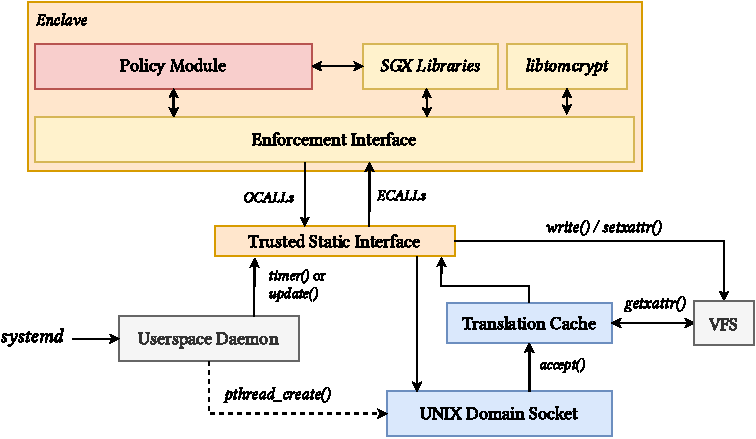
\includegraphics[width=\linewidth]{figures/EnclaveLayout.pdf}
    \caption{Abstract overview of an SGX enclave's protections.}
    \label{fig:sgx-basic}
\end{figure}


